%! TEX root = ../main.tex
% ==============================================================
% IMMUTABLE — generated automatically, do not edit this block
%
% — Provenance ───────────────────────────────────────────────────
%   script            : analysis_scratch/mooring_panel_freq_ka.py
%   computed_in       : analysis_scratch/mooring_panel_freq_ka.py (mooring_focus + damping_ka_fit data scopes overlaid)
%   plot_type         : mooring_panel_freq_ka
%   data_class        : DELEG
%   generated_at      : 2026-05-07T16:30:46
%   findings_doc      : 
%
% — Thesis context ──────────────────────────────────────────────
%   chapter           : 05
%   caption_label     : fig:ch05_mooring_panel_freq_ka
%   caption_short     : 
%
% — Filters ────────────────────────────────────────────────────
%   panel             : full, reverse
%   wind              : no, full
%   amplitude [V]     : 0.10, 0.20, 0.30
%   frequency [Hz]    : 1.30, 1.40, 1.50, 1.60
%   probes            : 
%   run_category      : 
%   quality_flag      : ok
%   mooring           : below_90_loose230, below_90_loose300, above_50
%
% — Data provenance ────────────────────────────────────────────
%   n_runs            : 
%   in_probes_used    : 
%   out_probes_used   : 
%   probe_configs     : 
%   non_final_config_n: 
%   datasets        :
%     PROCESSED-20251005-sixttry6roof-highMooring
%     PROCESSED-20251110-tett6roof-lowMooring
%     PROCESSED-20251110-tett6roof-lowMooring-2
%     PROCESSED-20251112-tett6roof
%     PROCESSED-20251113-tett6roof
%     PROCESSED-20251113-tett6roof-loosepaneltaped
%     PROCESSED-20251113-tett6roof-probeadjusted
%     PROCESSED-20260305-newProbePos-tett6roof
%     PROCESSED-20260306-newProbePos-tett6roof
%     PROCESSED-20260307-ProbPos4_31_FPV_2-tett6roof
%     PROCESSED-20260312-ProbPos4_31_FPV_2-tett6roof
%     PROCESSED-20260313-ProbePos4_31_FPV_2-tett6roof
%     PROCESSED-20260314-ProbePos4_31_FPV_2-tett6roof
%     PROCESSED-20260316-ProbePos4_31_FPV_2-tett6roof
%     PROCESSED-20260316-ProbePos4_31_FPV_2-tett6roof-under9Mooring
%     PROCESSED-20260319-ProbePos4_31_FPV_2-tett6roof-under9Mooring
%     PROCESSED-20260321-ProbePos4_31_FPV_2-tett6roof-under9Mooring-height100-RENAMED
%     PROCESSED-20260323-ProbePos4_31_FPV_2-tett6roof-under9Mooring-height100
%     PROCESSED-20260323-ProbePos4_31_FPV_2-tett6roof-under9Mooring-height136
%     PROCESSED-20260324-ProbePos4_31_FPV_2-tett6roof-under9Mooring-height100
%     PROCESSED-20260325-ProbePos4_31_FPV_2-tett6roof-under9Mooring-height100
%     PROCESSED-20260326-ProbePos4_31_FPV_2-tett6roof-under9Mooring-height100
%     PROCESSED-20260326-ProbePos4_31_FPV_2-tett6roof-under9Mooring-height100-lowrange
%     PROCESSED-20260327-ProbePos4_31_FPV_2-tett6roof-under9Mooring30-height100-lowrange
%   run_paths       :
%     (omitted — aggregate over > threshold runs, see datasets)
%
% — Method / numerical parameters ─────────────────────────────
%   grouper           : 
%   collapse_panels   : 
%   fft_window_hz     : 0.1
%   extra_params      : Union of two scopes: (A) 1.30 Hz, all folders, panel ∈ {full, reverse}, mooring ∈ {below_90 (loose230+loose300 lumped), above_50}; (B) 1.4–1.6 Hz, only canon-lowrange folders (20260326 + 20260327), panel = full, per_tag ∈ {per240, per40}, mooring = below_90. x = paddle-only ka per run = `IN Wavenumber (FFT)` × `IN Amplitude (FFT)` [m] — both factors FFT-measured, paddle-tone-only, NOT the wind-contaminated `IN ka (FFT)` pipeline column. Encoding: mooring × wind → colour (below_90 → WIND_COLOR_MAP, above_50 → cyan/pink); panel × freq → marker (normal panel uses `_freq_marker(amp, freq_idx)` cycling per freq; revers panel uses 6/5/4-point star at 1.30 Hz only). All hollow markers.
%
% — Summary stats cited in caption ────────────────────────────
%   stat:n_runs_total : 154
%   stat:n_at_1_30hz  : 104
%   stat:n_at_1_4_1_6hz : 50
%   stat:n_below_90   : 109
%   stat:n_above_50   : 45
%   stat:n_normal     : 131
%   stat:n_revers     : 23
%   stat:n_per_amp_A1 : 75
%   stat:n_per_amp_A2 : 39
%   stat:n_per_amp_A3 : 40
%
% — Subfigures available ───────────────────────────────────────
%     FIGURES/ch05_mooring_panel_freq_ka_A1.pdf
%     FIGURES/ch05_mooring_panel_freq_ka_A2.pdf
%     FIGURES/ch05_mooring_panel_freq_ka_A3.pdf
% ── end immutable block ─────────────────────────────────────────
\begin{figure}[p]
  \centering
  \begin{subfigure}[b]{1.0\linewidth}
    \centering
    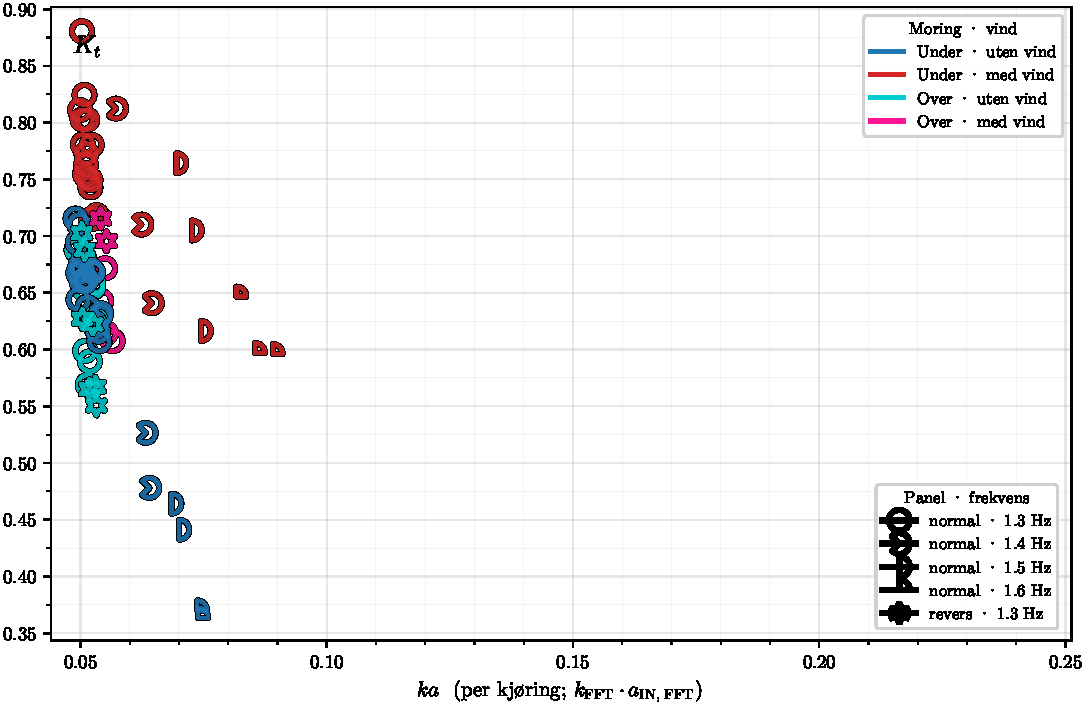
\includegraphics[width=\linewidth]{FIGURES/ch05_mooring_panel_freq_ka_A1.pdf}
    \caption{A1}
    \label{fig:ch05_mooring_panel_freq_ka_A1}
  \end{subfigure}
  \\[1ex]
  \begin{subfigure}[b]{1.0\linewidth}
    \centering
    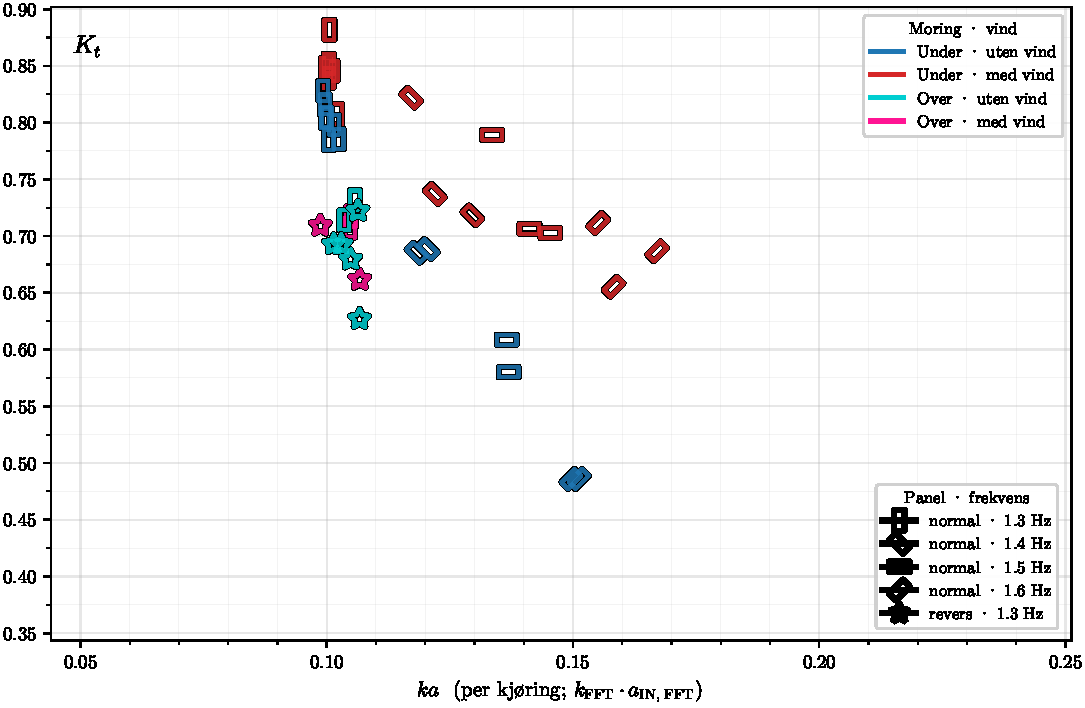
\includegraphics[width=\linewidth]{FIGURES/ch05_mooring_panel_freq_ka_A2.pdf}
    \caption{A2}
    \label{fig:ch05_mooring_panel_freq_ka_A2}
  \end{subfigure}
  \\[1ex]
  \begin{subfigure}[b]{1.0\linewidth}
    \centering
    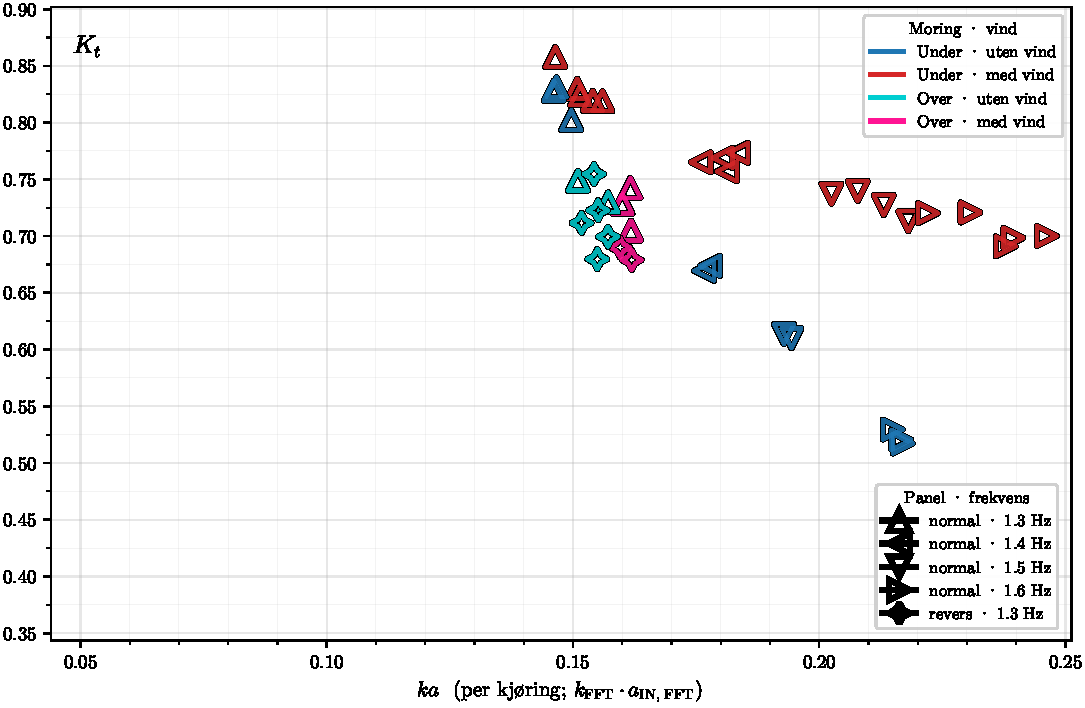
\includegraphics[width=\linewidth]{FIGURES/ch05_mooring_panel_freq_ka_A3.pdf}
    \caption{A3}
    \label{fig:ch05_mooring_panel_freq_ka_A3}
  \end{subfigure}
  \caption{
    % TODO: write caption
  }
  \label{fig:ch05_mooring_panel_freq_ka}
\end{figure}
